
\documentclass{article}
\usepackage[utf8]{inputenc}
\usepackage[english]{babel}
\usepackage[]{amsthm} %lets us use \begin{proof}
\usepackage[]{amssymb} %gives us the character \varnothing
\usepackage[]{setspace} %provides commands to set line spacing
\usepackage[left=0.75in, right=0.75in]{geometry}
\usepackage[colorlinks=true, linkcolor=blue, urlcolor=red, citecolor=blue]{hyperref}
\usepackage{xcolor}
\usepackage{soul}
\usepackage{amsmath}
\usepackage{amsfonts} % for \mathbb
\usepackage{amssymb}
\usepackage{graphicx}
\usepackage{float}
\usepackage{braket}





\begin{document}

\begin{center}
	\LARGE{Ansatz}\\[1em]
	\large Son Nguyen\\[1em]
	%\large \today
\end{center}

\noindent \href{https://journals.aps.org/prx/abstract/10.1103/PhysRevX.6.031007}{\textbf{Reference from Scalable Quantum Simulation of Molecular Energies}} \\
\tableofcontents
\newpage
We start with defining the Hamiltonian of the molecular Hydrogen.
\[H = g_0 \mathbb{I} + g_1 Z_0 + g_2 Z_1 + g_3 Z_0 Z_1 + g_4 Y_0 Y_1 + g_5 X_0 X_ 1\]
Where: $\{X_i, Z_i, Y_i\}$ denote the Pauli matrices acting on the i-th qubit and the real scalars $\{g_\gamma\}$ are efficiently computable functions of the hydrogen-hydrogen bond length R.
\[
	X = \begin{bmatrix}
		0 & 1 \\
		1 & 0
	\end{bmatrix} , \quad
	\mathbb{I} = \begin{bmatrix}
		1 & 0 \\
		0 & 1
	\end{bmatrix}, \quad
	Y = \begin{bmatrix}
		0 & -i \\
		i & 0
	\end{bmatrix}, \quad
	Z = \begin{bmatrix}
		1 & 0  \\
		0 & -1
	\end{bmatrix}
\]
\[g_0 \mathbb{I} = \begin{bmatrix}
		g_0 & 0   & 0   & 0   \\
		0   & g_0 & 0   & 0   \\
		0   & 0   & g_0 & 0   \\
		0   & 0   & 0   & g_0
	\end{bmatrix}, \quad
	g_1 Z_0 = \begin{bmatrix}
		g_1 & 0   & 0    & 0    \\
		0   & g_1 & 0    & 0    \\
		0   & 0   & -g_1 & 0    \\
		0   & 0   & 0    & -g_1
	\end{bmatrix}, \quad
	g_2 Z_1 = \begin{bmatrix}
		g_2 & 0    & 0   & 0    \\
		0   & -g_2 & 0   & 0    \\
		0   & 0    & g_2 & 0    \\
		0   & 0    & 0   & -g_2
	\end{bmatrix}, \quad
\]
\\
\[
	g_3 Z_0 Z_1 = \begin{bmatrix}
		g_3 & 0    & 0    & 0   \\
		0   & -g_3 & 0    & 0   \\
		0   & 0    & -g_3 & 0   \\
		0   & 0    & 0    & g_3
	\end{bmatrix}, \quad
	g_4 Y_0 Y_1 = \begin{bmatrix}
		0   & 0  & 0  & -g4 \\
		0   & 0  & g4 & 0   \\
		0   & g4 & 0  & 0   \\
		-g4 & 0  & 0  & 0
	\end{bmatrix}, \quad
	g_5 X_0 X_1 = \begin{bmatrix}
		0  & 0  & 0  & g5 \\
		0  & 0  & g5 & 0  \\
		0  & g5 & 0  & 0  \\
		g5 & 0  & 0  & 0
	\end{bmatrix}
\]
\\
\[
	H = \begin{bmatrix}
		g_0 + g_1 + g_2 + g_3 & 0                     & 0                     & g_5 - g_4              \\
		0                     & g_0 + g_1 - g_2 - g_3 & g_5 + g_4             & 0                      \\
		0                     & g_5 + g_4             & g_0 - g_1 + g_2 - g_3 & 0                      \\
		g_5 - g_4             & 0                     & 0                     & g_0 - g_1 - g_2 +  g_3
	\end{bmatrix}
\]
\section{Decomposing the UCCSD ansatz}
\begin{figure}[h]
	\label{fig:Figure 1}
	\centering
	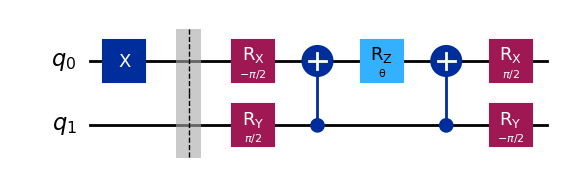
\includegraphics[width=0.8\textwidth, height=0.2\textheight]{Circ.png}
	\caption{The UCCSD ansatz for the Hydrogen molecule.}
\end{figure}

Reference state \(|10 \rangle\)
\begin{figure}[H]
	\centering
	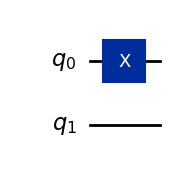
\includegraphics[width=0.2\textwidth, height=0.2\textheight]{ref.png}
\end{figure}
\[
	\left( X \otimes I\right) \cdot \left( |0 \rangle \otimes | 0 \rangle \right) = |10 \rangle
\]
\[
	\left(
	\begin{bmatrix}
			0 & 1 \\
			1 & 0
		\end{bmatrix}
	\otimes
	\begin{bmatrix}
			1 & 0 \\
			0 & 1
		\end{bmatrix}
	\right)
	\cdot
	\left(
	\begin{bmatrix}
			1 \\
			0
		\end{bmatrix}
	\otimes
	\begin{bmatrix}
			1 \\
			0
		\end{bmatrix}
	\right)
	=
	\begin{bmatrix}
		0 \\
		0 \\
		1 \\
		0
	\end{bmatrix}
\]

Apply parameterized ansatz
\begin{figure}[H]
	\centering
	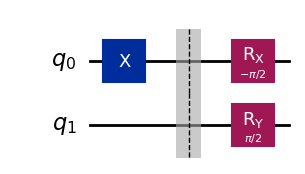
\includegraphics[width=0.3\textwidth, height=0.15\textheight]{ansatz1.png}
\end{figure}
\[
	\left(R_x(\frac{-\pi}{2}) \otimes R_y(\frac{\pi}{2})\right) \cdot |10 \rangle
\]

\[
	R_x(\frac{-\pi}{2}) = e^{-i X (\frac{-\pi}{4})} = \begin{bmatrix}
		\cos(\frac{-\pi}{4})   & -i\sin(\frac{-\pi}{4}) \\
		-i\sin(\frac{-\pi}{4}) & \cos(-\frac{\pi}{4})
	\end{bmatrix}
	=
	\begin{bmatrix}
		\frac{\sqrt{2}}{2}   & \frac{i \sqrt{2}}{2} \\
		\frac{i \sqrt{2}}{2} & \frac{\sqrt{2}}{2}
	\end{bmatrix}
\]

\[
	R_y(\frac{\pi}{2}) = e^{ -i Y(\frac{\pi}{4})} =
	\begin{bmatrix}
		\cos(\frac{\pi}{4}) & -\sin(\frac{\pi}{4}) \\
		\sin(\frac{\pi}{4}) & \cos(\frac{\pi}{4})
	\end{bmatrix} =
	\begin{bmatrix}
		\frac{\sqrt{2}}{2} & -\frac{\sqrt{2}}{2} \\
		\frac{\sqrt{2}}{2} & \frac{\sqrt{2}}{2}
	\end{bmatrix}
\]

\[
	\left(R_x(\frac{-\pi}{2}) \otimes R_y(\frac{\pi}{2})\right) =
	\begin{bmatrix}
		\frac{\sqrt{2}}{2}   & \frac{i \sqrt{2}}{2} \\
		\frac{i \sqrt{2}}{2} & \frac{\sqrt{2}}{2}
	\end{bmatrix}
	\otimes
	\begin{bmatrix}
		\frac{\sqrt{2}}{2} & -\frac{\sqrt{2}}{2} \\
		\frac{\sqrt{2}}{2} & \frac{\sqrt{2}}{2}
	\end{bmatrix} =
	\begin{bmatrix}
		\frac{1}{2} & \frac{-1}{2} & \frac{i}{2} & \frac{-i}{2} \\
		\frac{1}{2} & \frac{1}{2}  & \frac{i}{2} & \frac{i}{2}  \\
		\frac{i}{2} & \frac{-i}{2} & \frac{1}{2} & \frac{-1}{2} \\
		\frac{i}{2} & \frac{i}{2}  & \frac{1}{2} & \frac{1}{2}
	\end{bmatrix}
\]

\[
	\left(R_x(\frac{-\pi}{2}) \otimes R_y(\frac{\pi}{2})\right) \cdot |10 \rangle =
	\begin{bmatrix}
		\frac{1}{2} & \frac{-1}{2} & \frac{i}{2} & \frac{-i}{2} \\
		\frac{1}{2} & \frac{1}{2}  & \frac{i}{2} & \frac{i}{2}  \\
		\frac{i}{2} & \frac{-i}{2} & \frac{1}{2} & \frac{-1}{2} \\
		\frac{i}{2} & \frac{i}{2}  & \frac{1}{2} & \frac{1}{2}
	\end{bmatrix}
	\cdot
	\begin{bmatrix}
		0 \\
		0 \\
		1 \\
		0
	\end{bmatrix}
	=
	\begin{bmatrix}
		\frac{i}{2} \\
		\frac{i}{2} \\
		\frac{1}{2} \\
		\frac{1}{2} \\
	\end{bmatrix}
\]
The first CNOT (entanglement)
\begin{figure}[H]
	\centering
	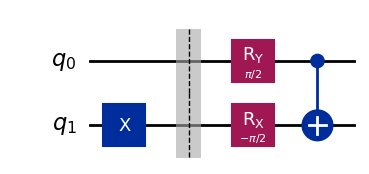
\includegraphics[width=0.3\textwidth, height=0.15\textheight]{1cnot.png}

\end{figure}
\[
	\begin{bmatrix}
		1 & 0 & 0 & 0 \\
		0 & 0 & 0 & 1 \\
		0 & 0 & 1 & 0 \\
		0 & 1 & 0 & 0
	\end{bmatrix}
	\cdot
	\begin{bmatrix}
		\frac{i}{2} \\
		\frac{i}{2} \\
		\frac{1}{2} \\
		\frac{1}{2} \\
	\end{bmatrix}
	=
	\begin{bmatrix}
		\frac{i}{2} \\
		\frac{1}{2} \\
		\frac{1}{2} \\
		\frac{i}{2} \\
	\end{bmatrix}
\]
The \(Z_\theta\) rotation gate:
\[
	Z_\theta = e^{-iZ(\frac{\theta}{2})} =
	\begin{bmatrix}
		e^{-i \frac{\theta}{2}} & 0                      \\
		0                       & e^{i \frac{\theta}{2}}
	\end{bmatrix}
\]

\[
	(Z_\theta \otimes I) \cdot \begin{bmatrix}
		\frac{i}{2} \\
		\frac{1}{2} \\
		\frac{1}{2} \\
		\frac{i}{2} \\
	\end{bmatrix} =
	\begin{bmatrix}
		e^{-i \frac{\theta}{2}} & 0                       & 0                      & 0                      \\
		0                       & e^{-i \frac{\theta}{2}} & 0                      & 0                      \\
		0                       & 0                       & e^{i \frac{\theta}{2}} & 0                      \\
		0                       & 0                       & 0                      & e^{i \frac{\theta}{2}}
	\end{bmatrix}
	\cdot
	\begin{bmatrix}
		\frac{i}{2} \\
		\frac{1}{2} \\
		\frac{1}{2} \\
		\frac{i}{2} \\
	\end{bmatrix} =
	\begin{bmatrix}
		\frac{\sin \left(\frac{\theta}{2}\right)}{2} + i \frac{\cos \left(\frac{\theta}{2}\right)}{2} \\
		\frac{\cos \left(\frac{\theta}{2}\right)}{2} - i \frac{\sin \left(\frac{\theta}{2}\right)}{2} \\
		\frac{\cos \left(\frac{\theta}{2}\right)}{2} + i \frac{\sin \left(\frac{\theta}{2}\right)}{2} \\
		\frac{-\sin \left(\frac{\theta}{2}\right)}{2} + i \frac{\cos \left(\frac{\theta}{2}\right)}{2}
	\end{bmatrix}
\]
The second CNOT (entanglement)
\[
	\begin{bmatrix}
		1 & 0 & 0 & 0 \\
		0 & 0 & 0 & 1 \\
		0 & 0 & 1 & 0 \\
		0 & 1 & 0 & 0
	\end{bmatrix}
	\cdot
	\begin{bmatrix}
		\frac{\sin \left(\frac{\theta}{2}\right)}{2} + i \frac{\cos \left(\frac{\theta}{2}\right)}{2} \\
		\frac{\cos \left(\frac{\theta}{2}\right)}{2} - i \frac{\sin \left(\frac{\theta}{2}\right)}{2} \\
		\frac{\cos \left(\frac{\theta}{2}\right)}{2} + i \frac{\sin \left(\frac{\theta}{2}\right)}{2} \\
		\frac{-\sin \left(\frac{\theta}{2}\right)}{2} + i \frac{\cos \left(\frac{\theta}{2}\right)}{2}
	\end{bmatrix}
	=
	\begin{bmatrix}
		\frac{\sin \left(\frac{\theta}{2}\right)}{2} + i \frac{\cos \left(\frac{\theta}{2}\right)}{2}  \\
		\frac{-\sin \left(\frac{\theta}{2}\right)}{2} + i \frac{\cos \left(\frac{\theta}{2}\right)}{2} \\
		\frac{\cos \left(\frac{\theta}{2}\right)}{2} + i \frac{\sin \left(\frac{\theta}{2}\right)}{2}  \\
		\frac{\cos \left(\frac{\theta}{2}\right)}{2} - i \frac{\sin \left(\frac{\theta}{2}\right)}{2}
	\end{bmatrix}
\]
The final rotation gates:
\[\left(R_x(\frac{\pi}{2}) \otimes R_y(\frac{-\pi}{2})\right) \cdot
	\begin{bmatrix}
		\frac{\sin \left(\frac{\theta}{2}\right)}{2} + i \frac{\cos \left(\frac{\theta}{2}\right)}{2}  \\
		\frac{-\sin \left(\frac{\theta}{2}\right)}{2} + i \frac{\cos \left(\frac{\theta}{2}\right)}{2} \\
		\frac{\cos \left(\frac{\theta}{2}\right)}{2} + i \frac{\sin \left(\frac{\theta}{2}\right)}{2}  \\
		\frac{\cos \left(\frac{\theta}{2}\right)}{2} - i \frac{\sin \left(\frac{\theta}{2}\right)}{2}
	\end{bmatrix}
\]

\[
	=
	\left(
	\begin{bmatrix}
			\cos \left(\frac{\pi}{4}\right)    & -i \sin \left(\frac{\pi}{4}\right) \\
			-i \sin \left(\frac{\pi}{4}\right) & \cos \left(\frac{\pi}{4}\right)
		\end{bmatrix}
	\otimes
	\begin{bmatrix}
			\cos \left(\frac{-\pi}{4}\right) & - \sin \left(\frac{-\pi}{4}\right) \\
			\sin \left(\frac{-\pi}{4}\right) & \cos \left(\frac{-\pi}{4}\right)
		\end{bmatrix}
	\right)
	\cdot
	\begin{bmatrix}
		\frac{\sin \left(\frac{\theta}{2}\right)}{2} + i \frac{\cos \left(\frac{\theta}{2}\right)}{2}  \\
		\frac{-\sin \left(\frac{\theta}{2}\right)}{2} + i \frac{\cos \left(\frac{\theta}{2}\right)}{2} \\
		\frac{\cos \left(\frac{\theta}{2}\right)}{2} + i \frac{\sin \left(\frac{\theta}{2}\right)}{2}  \\
		\frac{\cos \left(\frac{\theta}{2}\right)}{2} - i \frac{\sin \left(\frac{\theta}{2}\right)}{2}
	\end{bmatrix}
\]

\[
	=
	\left(
	\begin{bmatrix}
			\frac{1}{\sqrt{2}}  & \frac{-i}{\sqrt{2}} \\
			\frac{-i}{\sqrt{2}} & \frac{1}{\sqrt{2}}
		\end{bmatrix}
	\otimes
	\begin{bmatrix}
			\frac{1}{\sqrt{2}}  & \frac{1}{\sqrt{2}} \\
			\frac{-1}{\sqrt{2}} & \frac{1}{\sqrt{2}}
		\end{bmatrix}
	\right)
	\cdot
	\begin{bmatrix}
		\frac{\sin \left(\frac{\theta}{2}\right)}{2} + i \frac{\cos \left(\frac{\theta}{2}\right)}{2}  \\
		\frac{-\sin \left(\frac{\theta}{2}\right)}{2} + i \frac{\cos \left(\frac{\theta}{2}\right)}{2} \\
		\frac{\cos \left(\frac{\theta}{2}\right)}{2} + i \frac{\sin \left(\frac{\theta}{2}\right)}{2}  \\
		\frac{\cos \left(\frac{\theta}{2}\right)}{2} - i \frac{\sin \left(\frac{\theta}{2}\right)}{2}
	\end{bmatrix}
\]

\begin{equation}
	\label{eq:1}
	=
	\begin{bmatrix}
		\frac{1}{2}  & \frac{1}{2}  & \frac{-i}{2} & \frac{-i}{2} \\
		\frac{-1}{2} & \frac{1}{2}  & \frac{i}{2}  & \frac{-i}{2} \\
		\frac{-i}{2} & \frac{-i}{2} & \frac{1}{2}  & \frac{1}{2}  \\
		\frac{i}{2}  & \frac{-i}{2} & \frac{-1}{2} & \frac{1}{2}
	\end{bmatrix}
	\cdot
	\begin{bmatrix}
		\frac{\sin \left(\frac{\theta}{2}\right)}{2} + i \frac{\cos \left(\frac{\theta}{2}\right)}{2}  \\
		\frac{-\sin \left(\frac{\theta}{2}\right)}{2} + i \frac{\cos \left(\frac{\theta}{2}\right)}{2} \\
		\frac{\cos \left(\frac{\theta}{2}\right)}{2} + i \frac{\sin \left(\frac{\theta}{2}\right)}{2}  \\
		\frac{\cos \left(\frac{\theta}{2}\right)}{2} - i \frac{\sin \left(\frac{\theta}{2}\right)}{2}
	\end{bmatrix}
	=\begin{bmatrix}
		0                        \\
		- \sin(\frac{\theta}{2}) \\
		\cos(\frac{\theta}{2})   \\
		0
	\end{bmatrix}
\end{equation}
Reverse to match the qiskit ordering:
\begin{equation*}
	\begin{bmatrix}
		0                        \\
		\cos(\frac{\theta}{2})   \\
		- \sin(\frac{\theta}{2}) \\
		0
	\end{bmatrix}
	= |\phi(\vec{\theta}) \rangle = \cos\left(\frac{\theta}{2}\right) |01\rangle - \sin\left(\frac{\theta}{2}\right) |10\rangle
\end{equation*}
Use \(\theta = -3.37\):
\begin{equation*}
	\begin{bmatrix}
		0                       \\
		\cos(\frac{-3.37}{2})   \\
		- \sin(\frac{-3.37}{2}) \\
		0
	\end{bmatrix}
	\approx
	\begin{bmatrix}
		0       \\
		-0.1139 \\
		0.9935  \\
		0
	\end{bmatrix}
\end{equation*}
\textbf{*Note: This does not match the calculation, I had to switch place between the \(|01\rangle\) and \(|10\rangle\) to match the qiskit ordering}
\section{Unitary Couple Cluster Single Double (UCCSD)}
\subsection{Coupled Cluster Theory}
Couple Cluster theory was introduced for calculation nuclear binding energies. It is the gold standard for the balance between accucarcy and effiency. \\
Key concepts:
\begin{itemize}
	\item First quantization: individual particles are described by wavefucntion \(\psi(x)\) that satisfies the Schrodinger equation.
	\item Second quantization: instead of describing each particle separately, we define creation and annihilation operators that act on quantum states of an entire system.
\end{itemize}
The fundamental operators:
\begin{itemize}
	\item Creation operator: \(a^\dagger_i\) creates a particle in state \(i\).
	\item Annihilation operator: \(a_i\) removes a particle from state \(i\).
\end{itemize}
Fermionic Second Quantization: We described electron using second quantization.
\[\ket{\Psi} = a^\dagger_1 a^\dagger_3 \ket{0}\]
Which means we have occupied states 1 and 3 in the vaccum sate \(\ket{0}\).\\
\section{Quantum Tomography}
The expectation value (Quantum Tomography):
\hl{Using many measurements on identically prepared systems to get mean values of the some complete set of observables to reconstruct an estimate of the state. Quantum Tomography works to
	determine the state prior to the measurements.}\\

In this case, our state we want to reconstruct is \(|\phi(\vec{\theta})\rangle\).
\\
Starting with the denstiy matrix:
\begin{equation*}
	\rho = |\phi(\vec{\theta})\rangle \langle \phi(\vec{\theta})|
\end{equation*}
The general two qubits wavefunction can be written as:
\begin{equation*}
	| \phi \rangle = a_{00} |00\rangle + a_{01} |01\rangle + a_{10} |10\rangle + a_{11} |11\rangle
\end{equation*}
Where \(a_{ij} \in \mathbb{C}\), and \(\sum_{i,j} |a_{ij}|^2 = 1\). For our case, we have:
\begin{equation*}
	| \phi(\vec{\theta}) \rangle = \cos\left(\frac{\theta}{2}\right) |01\rangle - \sin\left(\frac{\theta}{2}\right) |10\rangle
\end{equation*}
Where: \(a_{00} = 0, a_{01} =\cos\left(\frac{\theta}{2}\right) , a_{10} = -\sin\left(\frac{\theta}{2}\right), a_{11} = 0 \), the goal is to reconstruct
\(a_{01}\) and \(a_{10}\). To achieve this, we need to make measurement in different basis. (X, Y, Z,\dots).
\\
\begin{figure}[H]
	\centering
	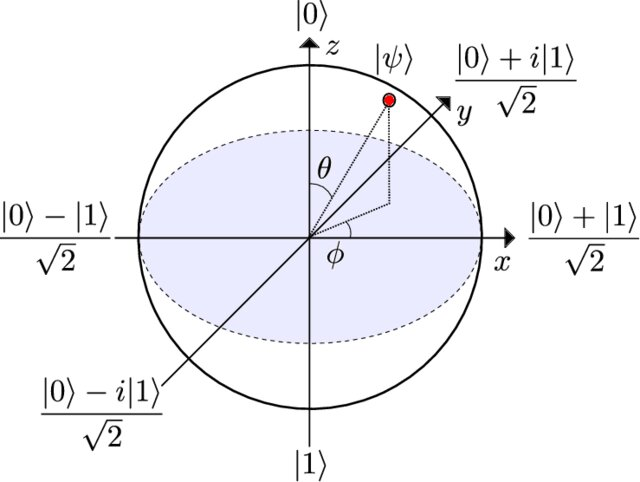
\includegraphics[width=0.55\textwidth, height=0.4\textheight]{The-Bloch-sphere-representation-of-a-qubit-The-basis-states-are-located-at-the-north-and_W640.jpg}
	\caption{\href{https://www.researchgate.net/publication/284259345_Quantum_optics_with_artificial_atoms/figures?lo=1}{Reference}}
\end{figure}
\noindent Let say we have a 1-qubit state \(| \psi \rangle = \alpha |0\rangle + \beta |1\rangle\). This state is a superposition of \(|0\rangle\) and \(|1\rangle\).\hl{ This is also called the $Z$ basis (computational basis).} \\ \\
Measurement in the $X$ basis - Diagonal basis/ Hadamard basis: superposition collapses the quantum state of the qubit \(|\psi\rangle\) to either \(|+\rangle\) or \(|-\rangle\).
\begin{align*}
	|+\rangle & = \frac{1}{\sqrt{2}}(|0\rangle + |1\rangle) \\
	|-\rangle & = \frac{1}{\sqrt{2}}(|0\rangle - |1\rangle) \\
	|0\rangle & = \frac{1}{\sqrt{2}}(|+\rangle + |-\rangle) \\
	|1\rangle & = \frac{1}{\sqrt{2}}(|+\rangle - |-\rangle) \\
\end{align*}
\begin{align}
	\label{eq:2}
	H |\psi\rangle & = H(\alpha |0\rangle + \beta |1\rangle)                                         \\
	               & = \alpha H|0\rangle + \beta H|1\rangle                                          \\
	               & = \alpha \begin{bmatrix}
		                          \frac{1}{\sqrt{2}} & \frac{1}{\sqrt{2}}  \\
		                          \frac{1}{\sqrt{2}} & -\frac{1}{\sqrt{2}}
	                          \end{bmatrix}
	\begin{bmatrix}
		1 \\
		0
	\end{bmatrix}
	+ \beta \begin{bmatrix}
		        \frac{1}{\sqrt{2}} & \frac{1}{\sqrt{2}}  \\
		        \frac{1}{\sqrt{2}} & -\frac{1}{\sqrt{2}}
	        \end{bmatrix}
	\begin{bmatrix}
		0 \\
		1
	\end{bmatrix}                                                                                   \\
	               & = \alpha \begin{bmatrix}
		                          \frac{1}{\sqrt{2}} \\
		                          \frac{1}{\sqrt{2}}
	                          \end{bmatrix}
	+
	\beta \begin{bmatrix}
		      \frac{1}{\sqrt{2}} \\
		      -\frac{1}{\sqrt{2}}
	      \end{bmatrix}                                                          \\
	               & = \alpha |+\rangle + \beta |-\rangle \quad \text{X basis}
\end{align}
Measurement in the $Y$ basis (Imaginary basis):
\begin{align*}
	(S^\dagger \cdot H) |\psi\rangle & = (S^\dagger \cdot H)(\alpha |0\rangle + \beta |1\rangle)                                                                  \\
	                                 & = \alpha (S^\dagger \cdot H)|0\rangle + \beta (S^\dagger \cdot H)|1\rangle                                                 \\
	                                 & = \alpha \begin{bmatrix}
		                                            \frac{1}{\sqrt{2}}  & \frac{1}{\sqrt{2}} \\
		                                            \frac{-i}{\sqrt{2}} & \frac{i}{\sqrt{2}}
	                                            \end{bmatrix}
	\cdot
	\begin{bmatrix}
		1 \\
		0
	\end{bmatrix}
	+ \beta \begin{bmatrix}
		        \frac{1}{\sqrt{2}}  & \frac{1}{\sqrt{2}} \\
		        \frac{-i}{\sqrt{2}} & \frac{i}{\sqrt{2}}
	        \end{bmatrix}
	\cdot
	\begin{bmatrix}
		0 \\
		1
	\end{bmatrix}                                                                                                                                                \\
	                                 & =
	\alpha \begin{bmatrix}
		       \frac{1}{\sqrt{2}} \\
		       \frac{-i}{\sqrt{2}}
	       \end{bmatrix}
	+
	\beta \begin{bmatrix}
		      \frac{1}{\sqrt{2}} \\
		      \frac{i}{\sqrt{2}}
	      \end{bmatrix}                                                                                                                       \\
	                                 & = \alpha \frac{1}{\sqrt{2}}(|0\rangle - i|1\rangle) + \beta \frac{1}{\sqrt{2}}(|0\rangle + i|1\rangle)\quad \text{Y basis}
\end{align*}
\begin{table}[H]
	\centering
	\begin{tabular}{|c|c|}
		\hline
		\textbf{Pauli Measurement} & \textbf{Unitary Transformation}                        \\
		\hline
		\(Z \otimes 1\)            & \(1 \otimes 1\)                                        \\
		\hline
		\(X \otimes 1\)            & \(H \otimes 1\)                                        \\
		\hline
		\(Y \otimes 1\)            & \(H S^\dagger \otimes 1\)                              \\
		\hline
		\(1 \otimes Z\)            & SWAP                                                   \\
		\hline
		\(1 \otimes X\)            & \((H \otimes 1)\)SWAP                                  \\
		\hline
		\(1 \otimes Y\)            & \((H S^\dagger \otimes 1)\)SWAP                        \\
		\hline
		\(Z \otimes Z\)            & \(\text{CNOT}_{10}\)                                   \\
		\hline
		\(X \otimes Z\)            & \(\text{CNOT}_{10} (H \otimes 1)\)                     \\
		\hline
		\(Y \otimes Z\)            & \(\text{CNOT}_{10} (H S^\dagger \otimes 1)\)           \\
		\hline
		\(Z \otimes X\)            & \(\text{CNOT}_{10} (1 \otimes H)\)                     \\
		\hline
		\(X \otimes X\)            & \(\text{CNOT}_{10} (H \otimes H)\)                     \\
		\hline
		\(Y \otimes X\)            & \(\text{CNOT}_{10} (H S^\dagger \otimes H)\)           \\
		\hline
		\(Z \otimes Y\)            & \(\text{CNOT}_{10} (1 \otimes H S^\dagger)\)           \\
		\hline
		\(X \otimes Y\)            & \(\text{CNOT}_{10} (H \otimes H S^\dagger)\)           \\
		\hline
		\(Y \otimes Y\)            & \(\text{CNOT}_{10} (H S^\dagger \otimes H S^\dagger)\) \\
		\hline
	\end{tabular}
\end{table}
\begin{equation*}
	\langle H \rangle = g_0 \mathbb{I} + g_1 \langle Z_0 \rangle + g_2 \langle Z_1 \rangle + g_3 \langle Z_0 Z_1 \rangle + g_4 \langle Y_0 Y_1 \rangle + g_5 \langle X_0 X_1 \rangle
\end{equation*}
\begin{equation*}
	\langle P \rangle = \sum_{\text{bitstring}}  (-1)^{\text{parity}} \left( \frac{\text{count}}{\text{shots}} \right)
\end{equation*}
Where:
\begin{itemize}
	\item parity = bitstring.count('1') mod 2
	\item count = number of times the bitstring was measured
	\item shots = total number of measurements
\end{itemize}
\subsection{Theoretical Analysis (XX)}
\begin{itemize}
	\item For the \(XX\) operator
	      \begin{equation*}
		      XX =
		      \begin{bmatrix}
			      0 & 1 \\
			      1 & 0
		      \end{bmatrix}
		      \otimes
		      \begin{bmatrix}
			      0 & 1 \\
			      1 & 0
		      \end{bmatrix}
		      = \begin{bmatrix}
			      0 & 0 & 0 & 1 \\
			      0 & 0 & 1 & 0 \\
			      0 & 1 & 0 & 0 \\
			      1 & 0 & 0 & 0
		      \end{bmatrix}
	      \end{equation*}

	      The expectation value of an observable \(O\) is given by:
	      \begin{equation*}
		      \langle O \rangle = \sum_{i} \lambda_i p_i
	      \end{equation*}
	      Where \(p_i\) is the probability of measuring the state in the \(i^{th}\) eigenstate. $\lambda_i$ is the expectation value correspoding to eigenstate.\\ \\
	      From equation \eqref{eq:2} we can see that \(H |0 \rangle = | + \rangle, H|1\rangle = | - \rangle\). The corresponding eigenvalues for the operator \(X\) are
	      \[\langle + | X |+ \rangle = 1 \text{ and } \langle - | X | - \rangle = -1\]
	      For the 2 qubit states, we have:
	      \[(H \otimes H)|00\rangle = \begin{bmatrix}
			      \frac{1}{2} \\
			      \frac{1}{2} \\
			      \frac{1}{2} \\
			      \frac{1}{2}
		      \end{bmatrix} = |++\rangle = \frac{1}{2}(|00\rangle + |01\rangle + |10\rangle + |11\rangle)\]
	      \[(H \otimes H)|01\rangle =|+-\rangle = \frac{1}{2}(|00\rangle - |01\rangle +|10\rangle -|11\rangle)\]
	      \[(H \otimes H)|10\rangle =|-+\rangle = \frac{1}{2} (|00\rangle + |01\rangle - |10\rangle - |11\rangle)\]
	      \[(H \otimes H)|11\rangle =|--\rangle\]
	      Apply the operator \(XX\) on each state:
	      \begin{align*}
		      XX|++\rangle & = \frac{1}{2}(XX|00\rangle + XX|01\rangle + XX|10\rangle + XX|11\rangle)                       \\
		                   & = \frac{1}{2}(|11\rangle + |10\rangle + |01\rangle + |00\rangle) = |++\rangle                  \\
		                   & \Rightarrow \langle++ |XX|++ \rangle = \langle++ |++ \rangle =1                                \\
		      XX|+-\rangle & = \frac{1}{2}(XX|00\rangle - XX|01\rangle + XX|10\rangle - XX|11\rangle)                       \\
		                   & = \frac{1}{2}(|11\rangle - |10\rangle + |01\rangle - |00\rangle) = \frac{1}{2} \begin{bmatrix}
			                                                                                                    -1 \\
			                                                                                                    1  \\
			                                                                                                    -1 \\
			                                                                                                    1
		                                                                                                    \end{bmatrix}  \\
		                   & \Rightarrow \langle+- |XX|+- \rangle = \begin{bmatrix}
			                                                            \frac{1}{2} & \frac{-1}{2} & \frac{1}{2} & \frac{-1}{2}
		                                                            \end{bmatrix}\cdot \begin{bmatrix}
			                                                                               \frac{-1}{2} \\
			                                                                               \frac{1}{2}  \\
			                                                                               \frac{-1}{2} \\
			                                                                               \frac{1}{2}
		                                                                               \end{bmatrix} = -1
	      \end{align*}
	      and so we can get the remaining expectation values \(\langle -+ |XX| -+\rangle = -1, \langle -- |XX|--\rangle = 1\)
	      \begin{table}[H]
		      \centering
		      \begin{tabular}{|c|c|c|}
			      \hline
			      \text{Measurement} & \text{XX basis equivalent} & \text{XX Expectation Value} \\
			      \hline
			      $|00\rangle$       & $|++\rangle$               & 1                           \\
			      \hline
			      $|01\rangle$       & $|+-\rangle$               & -1                          \\
			      \hline
			      $|10\rangle$       & $|-+\rangle$               & -1                          \\
			      \hline
			      $|11\rangle$       & $|--\rangle$               & 1                           \\
			      \hline
		      \end{tabular}
	      \end{table}

\end{itemize}
\subsection{Experimental Analysis (XX)}
From our circuit that produce the wavefunction \(|\phi(\vec{\theta})\rangle\) (see Figure \ref{fig:Figure 1}). We just need to apply two Hadamard gates to the qubits and measure the expectation value of the \(XX\) operator.
\begin{figure}[H]
	\label{fig:Figure XX}
	\centering
	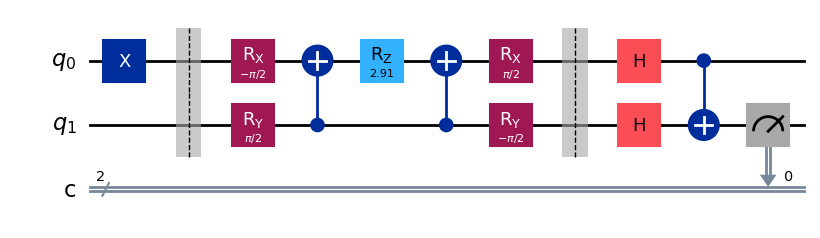
\includegraphics[width=0.7\textwidth, height=0.2\textheight]{XX.png}
	\caption{Circuit for the \(XX\) operator}
\end{figure}
\noindent Give the trial wavefunction \(|\phi(\vec{\theta})\rangle = \cos\left(\frac{\theta}{2}\right)|01\rangle - \sin\left(\frac{\theta}{2}\right)|10\rangle\). Applying the Hadamard gates given:
\begin{align*}
	 & (H \otimes H)|\phi(\vec{\theta})\rangle                                                                                                                                                                                                                                                                    \\
	 & = (H \otimes H)(\cos\left(\frac{\theta}{2}\right)|01\rangle - \sin\left(\frac{\theta}{2}\right)|10\rangle)                                                                                                                                                                                                 \\
	 & =  \cos\left(\frac{\theta}{2}\right)(H|0\rangle \otimes H|1\rangle) - \sin\left(\frac{\theta}{2}\right)(H|1\rangle \otimes H|0\rangle)                                                                                                                                                                     \\
	 & = \cos\left(\frac{\theta}{2}\right)\left[\frac{1}{\sqrt{2}}(|0\rangle+|1\rangle) \otimes \frac{1}{\sqrt{2}}(|0\rangle - |1\rangle)\right] - \sin\left(\frac{\theta}{2}\right)\left[\frac{1}{\sqrt{2}}(|0\rangle - |1\rangle) \otimes \frac{1}{\sqrt{2}}(|0\rangle + |1\rangle)\right]                      \\
	 & = \cos\left(\frac{\theta}{2}\right)\left[\frac{1}{2}(|00\rangle - |01\rangle + |10\rangle - |11\rangle)\right] - \sin\left(\frac{\theta}{2}\right)\left[\frac{1}{2}(|00\rangle + |01\rangle - |10\rangle - |11\rangle)\right]                                                                              \\
	 & = \frac{1}{2}\left\{\left[\cos\left(\frac{\theta}{2}\right) - \sin\left(\frac{\theta}{2}\right)\right]\ket{00} - \left[\cos\left(\frac{\theta}{2}\right) + \sin\left(\frac{\theta}{2}\right)\right] \ket{01} + \left[\cos\left(\frac{\theta}{2}\right) + \sin\left(\frac{\theta}{2}\right)\right] \ket{10}
	+ \left[\sin\left(\frac{\theta}{2}\right)- \cos\left(\frac{\theta}{2}\right) \right]\ket{11} \right\}                                                                                                                                                                                                         \\
\end{align*}
Then we apply the \(\text{CNOT}_{01}\) gate to the state:
\begin{align*}
	 & \text{CNOT}_{01} \left\{\cos\left(\frac{\theta}{2}\right)\left[\frac{1}{2}(|00\rangle - |01\rangle + |10\rangle - |11\rangle)\right] - \sin\left(\frac{\theta}{2}\right)\left[\frac{1}{2}(|00\rangle + |01\rangle - |10\rangle - |11\rangle)\right]\right\}                                                \\
	 & = \cos\left(\frac{\theta}{2}\right)\left[\frac{1}{2}\text{CNOT}_{01}(|00\rangle - |01\rangle + |10\rangle - |11\rangle)\right] - \sin\left(\frac{\theta}{2}\right)\left[\frac{1}{2}\text{CNOT}_{01}(|00\rangle + |01\rangle - |10\rangle - |11\rangle)\right]                                              \\
	 & = \cos\left(\frac{\theta}{2}\right)\left[\frac{1}{2}(|00\rangle - |01\rangle + |11\rangle - |10\rangle)\right] - \sin\left(\frac{\theta}{2}\right)\left[\frac{1}{2}(|00\rangle + |01\rangle - |11\rangle - |10\rangle)\right]                                                                              \\
	 & = \frac{1}{2}\left\{\left[\cos\left(\frac{\theta}{2}\right) - \sin\left(\frac{\theta}{2}\right)\right]\ket{00} - \left[\cos\left(\frac{\theta}{2}\right) + \sin\left(\frac{\theta}{2}\right)\right] \ket{01} + \left[\sin\left(\frac{\theta}{2}\right) - \cos\left(\frac{\theta}{2}\right)\right] \ket{10}
	+ \left[\sin\left(\frac{\theta}{2}\right)+ \cos\left(\frac{\theta}{2}\right) \right]\ket{11} \right\}
\end{align*}
After applying \(\text{CNOT}_{01}\) gate.
\[\underbrace{\ket{00}}_{even} \rightarrow \ket{0\textcolor{red}{0}}; \; \underbrace{\ket{01}}_{odd} \rightarrow \ket{0\textcolor{blue}{1}}; \; \underbrace{\ket{10}}_{odd} \rightarrow \ket{1 \textcolor{blue}{1}}; \; \underbrace{\ket{11}}_{even} \rightarrow \ket{1\textcolor{red}{0}}\]
We can see that after applying the \(\text{CNOT}_{01}\) gate, the second qubit is flipped (the colored). Now measuring just the second qubit give us the parity of the state. If the parity is even we will see 0 and if the parity is odd we will see 1. A CNOT gate is used to compute the parity
of two qubits and store it in one qubit without fully collapsing the state. \\
\section{Bell Measurement (Incomplete)}
Alternatively, using Bell Measurement to reconstruct the trial wavefunction with the parameter \(\theta \approx -3.37\), getting the expectation after 1000 measurements:
\begin{figure}[H]
	\centering
	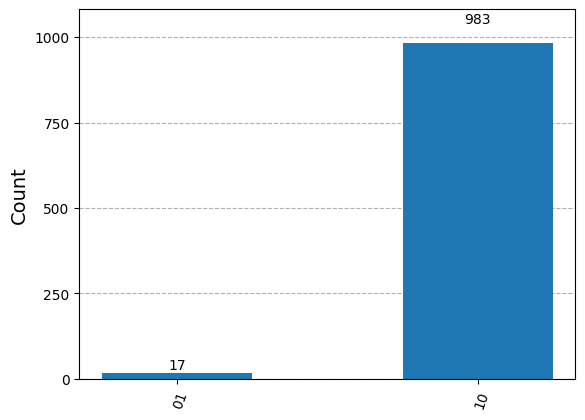
\includegraphics[width=0.5\textwidth, height=0.3\textheight]{1000.png}
\end{figure}

From the figure, we have see there is \(1.7 \% \) of \(|01\rangle\) and \(98.3 \%\) of \(|10\rangle\).
\begin{align*}
	\sqrt{1.7 \% }|01\rangle + \sqrt{98.3 \%}|10\rangle & = |\phi(\vec{\theta}) \rangle \\
	\pm 0.13|01\rangle \pm 0.99  |10\rangle             & = |\phi(\vec{\theta}) \rangle
\end{align*}
To determine the sign of our trial wavefunction, we can use Bell measurements. We can measures any state which is an superposition of \(|00\rangle, |01\rangle, |10\rangle , |11\rangle\) in the Bell basis.
\begin{align*}
	|\Phi^+\rangle & = \frac{1}{\sqrt{2}}(|00\rangle + |11\rangle) \\
	|\Phi^-\rangle & = \frac{1}{\sqrt{2}}(|00\rangle - |11\rangle) \\
	|\Psi^+\rangle & = \frac{1}{\sqrt{2}}(|01\rangle + |10\rangle) \\
	|\Psi^-\rangle & = \frac{1}{\sqrt{2}}(|01\rangle - |10\rangle)
\end{align*}
By combining a CNOT gate followed by a Hadamard gate, we can measure the state in the Bell basis.
\begin{align*}
	U |\Phi^+\rangle & = |00\rangle \\
	U |\Phi^-\rangle & = |01\rangle \\
	U |\Psi^+\rangle & = |10\rangle \\
	U |\Psi^-\rangle & = |11\rangle
\end{align*}
Where \(U_{Bell} = \left( H \otimes I \right) \cdot \text{CNOT}(0,1)\)
\begin{equation*}
	U_{Bell} = \frac{1}{\sqrt{2}}\begin{bmatrix}
		1 & 0  & 0 & 1  \\
		1 & 0  & 0 & -1 \\
		0 & 1  & 1 & 0  \\
		0 & -1 & 1 & 0
	\end{bmatrix}
\end{equation*}
Applying the \(U_{Bell}\) on \(\begin{bmatrix}
	A \\
	B \\
	C \\
	D
\end{bmatrix}\)
\begin{equation*}
	U_{Bell} \cdot \begin{bmatrix}
		A \\
		B \\
		C \\
		D
	\end{bmatrix}
	=
	\frac{1}{\sqrt{2}}\begin{bmatrix}
		A + D \\
		A-D   \\
		B+C   \\
		B - C
	\end{bmatrix}
\end{equation*}
\begin{figure}[H]
	\centering
	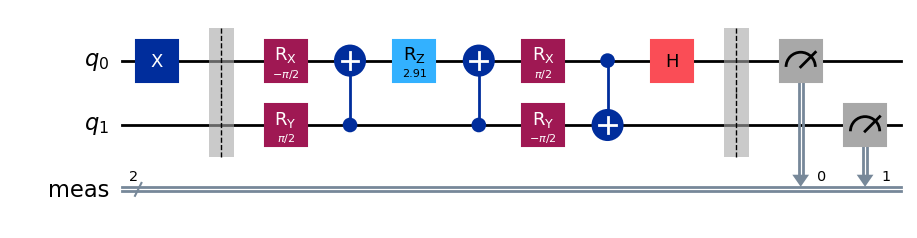
\includegraphics[width=0.9\textwidth, height=0.25\textheight]{BellM.png}
\end{figure}
The trial wavefunction after applying the \(U_{Bell}\) unitary gate:
\begin{equation*}
	U_{Bell} \cdot |\phi(\vec{\theta})\rangle = U_{Bell} \cdot \begin{bmatrix}
		0                                  \\
		\cos\left(\frac{\theta}{2}\right)  \\
		-\sin\left(\frac{\theta}{2}\right) \\
		0
	\end{bmatrix}
	= \frac{1}{\sqrt{2}}
	\begin{bmatrix}
		0                                                                     \\
		0                                                                     \\
		\cos\left(\frac{\theta}{2}\right) - \sin\left(\frac{\theta}{2}\right) \\
		\cos\left(\frac{\theta}{2}\right) + \sin\left(\frac{\theta}{2}\right)
	\end{bmatrix}
	\begin{array}{c}
		|00 \rangle \\
		|01 \rangle \\
		|10 \rangle \\
		|11 \rangle
	\end{array}
	\begin{array}{c}
		\\
		\\
		\approx 0.39\% \\
		\approx 0.61\%
	\end{array}
\end{equation*}
Using \(\theta \approx -3.37\) we have:
\begin{figure}[H]
	\centering
	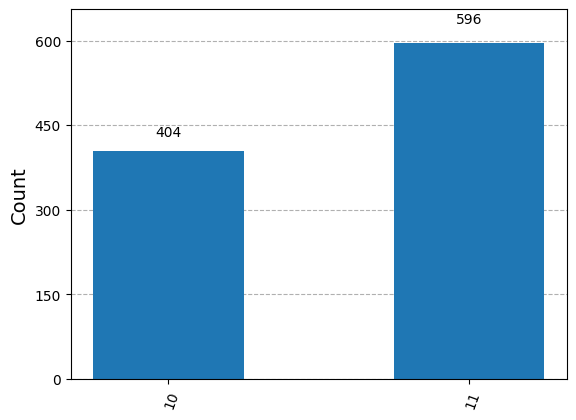
\includegraphics[width=0.5\textwidth, height=0.3\textheight]{BellHis.png}
\end{figure}
We can see the counts of \(|11\rangle\) is dominant, which means the state is \(|\Psi^-\rangle\). Therefore, the sign between \(|01\rangle\) and \(|10\rangle\) is negative.
\begin{equation}
	0.13|01\rangle - 0.99 |10\rangle = |\phi(\vec{\theta}) \rangle
\end{equation}
\href{https://grishmaprs.medium.com/measurement-based-quantum-computation-9de426f40856}{\hl{Reference}}.


Now we plug in the \(\theta\) to equation \eqref{eq:1} to compare with equation (2), we have:
\begin{align*}
	-\sin\left(\frac{-3.37}{2}\right) |01 \rangle + \cos\left(\frac{-3.37}{2}\right) |10 \rangle & = |\phi(\vec{\theta}) \rangle \\
	0.993 |01\rangle  - 0.11 |10\rangle                                                          & = |\phi(\vec{\theta}) \rangle
\end{align*}

\begin{center}
	\textbf{There is a mistake for my bell measurement, I will correct it later.}
\end{center}

\section{Cost Function}
\hl{Mathematically we can use the Hamiltonian and the trial wavefunction, we can get our cost function (energy) as:}
\[E = \langle \phi({\vec{\theta}})| H | \phi(\vec{\theta}) \rangle\]
\[
	\begin{bmatrix}
		0 & \cos(\frac{\theta}{2}) & -\sin(\frac{\theta}{2}) & 0
	\end{bmatrix}
	\cdot
	\begin{bmatrix}
		g_0 + g_1 + g_2 + g_3 & 0                     & 0                     & g_5 - g_4              \\
		0                     & g_0 + g_1 - g_2 - g_3 & g_5 + g_4             & 0                      \\
		0                     & g_5 + g_4             & g_0 - g_1 + g_2 - g_3 & 0                      \\
		g_5 - g_4             & 0                     & 0                     & g_0 - g_1 - g_2 +  g_3
	\end{bmatrix}
	\cdot
	\begin{bmatrix}
		0                        \\
		\cos(\frac{\theta}{2})   \\
		- \sin(\frac{\theta}{2}) \\
		0
	\end{bmatrix}
\]

Plug in  \(g_0 = -0.4804, g_1 = 0.3435, g_2 = -0.4347, g_3 = 0.5716, g_4 = 0.091, g_5 = 0.091\) we have:
\[
	\begin{bmatrix}
		0 & \cos(\frac{\theta}{2}) & -\sin(\frac{\theta}{2}) & 0
	\end{bmatrix}
	\cdot
	\begin{bmatrix}
		0 & 0       & 0       & 0      \\
		0 & -0.2738 & 0.182   & 0      \\
		0 & 0.182   & -1.8302 & 0      \\
		0 & 0       & 0       & 0.1824
	\end{bmatrix}
	\cdot
	\begin{bmatrix}
		0                        \\
		\cos(\frac{\theta}{2})   \\
		- \sin(\frac{\theta}{2}) \\
		0
	\end{bmatrix}
	\approx \text{\hl{$-1.851 \quad (\text{with } \theta = -3.37)$}}
\]


The minimum energy can be found using classical optimization techniques.

\[E_{min} = \langle \phi_{min}(\vec{\theta}) \mid H \mid \phi_{min}(\vec{\theta}) \rangle\]


\end{document}